%\documentclass[8pt,letterpaper,twocolumn]{article} % TODO: twocolumn if it fits nicely
\documentclass[8pt,letterpaper]{article}
\usepackage{graphicx}
\usepackage{fullpage}
\usepackage{setspace}
\usepackage{algorithm}
\usepackage{algorithmic}
\usepackage{amsmath} % for dfrac
\usepackage{enumerate} % for letter-based enumerations

\addtolength{\textwidth}{2cm}
\addtolength{\hoffset}{-1cm}
\addtolength{\textheight}{2cm}
\addtolength{\voffset}{-2cm}

\begin{document} % All chapter & section references are for "Stewart Calculus 7th edition - ET"

% TODO: Common derivatives & anti-derivatives (see front of Tan's Calculus book)

\section{Differentiation Rules}

\subsection*{Product rule}
\begin{equation}
(f\cdot g)'=f'\cdot g+f\cdot g' \,\! 
\end{equation}

\subsection*{Quotient rule}
\begin{equation}
\frac{d}{dx} \frac{f}{g} = \frac{f'g - fg'}{g^2}
\end{equation}

\subsection*{Chain rule}
\begin{equation}
\frac{d}{dx} f(g(x)) = f'(g(x))g'(x)
\end{equation}
Examples: \\
$\frac{d}{dx} \sin 2x = \cos 2x * 2 = 2 \cos 2x$ \\
$\frac{d}{dx} \ln(x^{\frac{5}{3}}) = \frac{5}{3} x^{\frac{2}{3}} \frac{1}{x^{5/3}} = \frac{5}{3x}$ \\

\subsection*{L'Hopital's rule}
l'Hopital's rule uses derivatives to help evaluate limits involving indeterminate forms
(e.g. $0^0,\, \frac{0}{0},\, 1^\infty,\, \infty - \infty,\, \frac{\infty}{\infty},\,
0 \cdot \infty,\, \infty^0$)
\begin{equation}
\lim_{x \to x_0} \frac{f(x)}{g(x)} = \lim_{x \to x_0} \frac{f'(x)}{g'(x)}
\end{equation}

% What is integration
% dx means "w.r.t to x" i.e. integrating for x
% f(x) = "f of x"
% f'(x) = "f prime of x" which is the same as f(x) d/dx, meaning you have to derive it.
% \[ \int y\, \mathrm{d}x \] = "(definite) integral of y of x"
% \[ \int_a^b y\, \mathrm{d}x \] = "(indefinite) integral of y of x from a to b"

\begin{table}
	\begin{tabular}{ l l } % Note: using a tabular environment places math in inline mode.
	$\int c f(x) \, dx = c \int f(x) \, dx$ &
	$\int [f(x) + g(x)] \, dx = \int f(x) \, dx + \int g(x) \, dx$ \\[5pt]
	
	$\int k\,dx = k\,x + C$ & 
	$\int \tan\,x \, dx = \ln | \sec\,x | + C$ \\[5pt]
	
	$\int x^n\,dx = \frac{1}{n+1}\,x^{n+1} + C \; (n \neq -1)$ &
	$\int x^{-1} \, dx = \int \frac{1}{x} \, dx = \ln|x| + C$ \\[5pt]
	
  $\int e^x \, dx = e^x + C$ &
  $\int a^x \, dx = \frac{a^x}{\ln \, a} + C$\\[5pt]	
	
  $\int \sin x \, dx = -\cos x + C$ &
  $\int \cos x \, dx = \sin x + C$ \\[5pt]
  
  $\int \sec^2x \, dx = \tan x + C$ &
  $\int \csc^2x \, dx = -\cot x + C$ \\[5pt]

  $\int \sec x \; \tan x \, dx = \sec x + C$ &
  $\int \csc x \; \cot x \, dx = -\csc x + C$ \\[5pt]
  
  $\int \frac{1}{1 + x^2} \, dx = \arctan x + C$ &
  $\int \frac{1}{\sqrt{1-x^2}} \, dx = \arcsin x + C$ \\[5pt]
  
%  $\int \, dx = + C$ &
%  $\int \, dx = + C$ \\[5pt]
  
%  $\int \, dx = + C$ &
%  $\int \, dx = + C$ \\[5pt]	
	\end{tabular}
	\caption{Common Indefinite Integrals} % See page 398 (7th ed.)
\end{table}

\section{Applications of Integration} % chapter 6
  % Definite Integrals
  % Indefinite Integrals --> area under a curve from a to b
  % TIP: Place independent constants outside the integral!
    % e.g. \int 2x dx = 2 \int x dx


\subsection*{Area between Curves} % Section 6.1
  % A = \int_a^b f(x) - g(x) dx, where f(x) is on top
  % hint: sometimes easier to integrate w.r.t. y

\subsection*{Volumes} % Section 6.2
\emph{TODO} \\
\begin{eqnarray*}
V &=& \int_a^b A(x) \, dx \\
V_{disk} &=& \pi \int_a^b (radius)^2 \, dx \\
V_{washer} &=& \pi \int_a^b (outer\:radius)^2 - (inner\:radius)^2 \, dx \\
\end{eqnarray*}
$V_{disk} = \pi \int_a^b \, [f(x)]^2 \, dx$ \\
$V_{washer} = \pi \int_a^b (outer\:radius)^2 - (inner\:radius)^2 \, dx$ \\

When rotating from an axis that's not the x-axis (integrating w.r.t. x)
then you have to negate the difference as if it was being rotated about the x-axis
by either adding or subtracting the difference in your inner and outer radiuses.

\subsection*{Average Value of a Function} % Section 6.5
$f_{avg} = \frac{1}{b-a} \int_a^b f(x) \, dx$

\section{Techniques of Integration} % Section 7...? (See notes)
% => Simplify
% => Obvious substitution
% => Classify: Trig integral / Rational / IBP / IBTS ?
% => Try again (different sub, trig identity, multiple methods, etc.)

\subsection*{Integration by Parts (IBP)} % Section 7.1
\begin{equation}
\int u \, dv = uv - \int v \, du
\end{equation}
Use when $u$-substitution doesn't work.
Some examples when you would use IBP:
\begin{tabular}{l l}
$\int \ln x \, dx$ & $\int e^{-\theta} \cos 2\theta \, d\theta$ \\ 
$\int \arcsin x \, dx$ & $\int \arctan x \, dx$ \\ 
\end{tabular} 

% Definite integrals using IBP
% Reverse product rule
% Reverse chain rule
% Integration by u-substitution (for integrating only -- use if chain rule used for deriving)
  % e.g. \int sin(2x) dx = 1/2 \int sin u du = 1/2 (-cos u) = -1/2 cos(2x) + constant
  % u = 2x, du = 2dx, dx = 1/2 du

\subsection*{Trigonometric Integrals} % (section 7.2)
% TODO: tangent and cotangent IDs, half angle formulas, reciprocal identities
\begin{table}
\begin{tabular}{l l}
$\sin^2 \theta + \cos^2 \theta = 1$ \\
$\tan^2 \theta + 1 = \sec^2 \theta$ \\ 
$1 + \cot^2 \theta = \csc^2 \theta$
\end{tabular}
\caption{Pythagorean Identities}
\end{table}

\subsection*{Trigonometric Substitution} % (7.3 in Stewart, 6.3 in Tan)

\begin{enumerate} % TODO: put all extra info as nested bullet points
\item Check if u-substitution is more appropriate (e.g. $\int x \sqrt{4-x^2}\,dx$)
\item Substitute the expression (3 options)
\item Simplify the expression (eliminate terms and square root using trig identities)
\item Integrate when possible (remember to put constants outside)
\item Draw a right-angled triangle and label with trig ratio of the substitution trig function
\begin{itemize}
\item $\sin \theta = \frac{opp}{hyp}$, $\:\cos \theta = \frac{adj}{hyp}$, $\:\tan \theta = \frac{opp}{adj}$
\item $\cot \theta = \frac{1}{\tan \theta} = \frac{adj}{opp}$, $\:\sec \theta = \frac{1}{\cos \theta} = \frac{hyp}{adj}$, $\:\csc \theta = \frac{1}{\sin \theta} = \frac{hyp}{opp}$
\end{itemize}
\item Substitute back for $\theta$ (return to original variable $x$)
\begin{itemize}
\item Find $\theta$ if leftover on its own. \\
e.g. $x = 3 \sin \theta \Rightarrow \sin \theta = \frac{x}{3} \Rightarrow \theta = \arcsin (\frac{x}{3}) = \sin^{-1} (\frac{x}{3})$
\item Find substitutions for leftover trig functions. \\
e.g. $\frac{1}{16} \sin \theta + C$ is the non-final answer. Substitution was $t = 4 \sec \theta \Rightarrow \sec \theta = \frac{t}{4} = \frac{hyp}{adj}$. Draw a right-angled triangle.
Find $\sin \theta = \frac{opp}{hyp} = \frac{\sqrt{t^2-16}}{t}$. Final answer is $\frac{\sqrt{t^2-16}}{16t} + C$.

\end{itemize}
\end{enumerate}

\begin{tabular}{|c|c|c|}
\hline 
Expression & Substitution & Identity \\
\hline
$\sqrt{a^2 - x^2}$ &
$x = a \sin \theta$, $dx = a \cos \theta$ & %$-\frac{\pi}{2} \leq \theta \leq \frac{\pi}{2}$ &
$1 - \sin^2\theta = \cos^2\theta$
\\
$\sqrt{a^2 + x^2}$ &
$x = a \tan \theta$, $dx = a \sec^2 \theta$ & %$-\frac{\pi}{2} < \theta < \frac{\pi}{2}$ &
$1 + \tan^2\theta = \sec^2\theta$
\\ 
$\sqrt{x^2 - a^2}$ &
$x = a \sec \theta$, $dx = a \sec \theta \: \tan \theta$ & %$0 \leq \theta < \frac{\pi}{2}$ or $\pi \leq \theta < \frac{3\pi}{2}$ &
$\sec^2\theta - 1 = \tan^2\theta$
\\ 
\hline 
\end{tabular} 

\begin{figure}[hbtp]
\caption{Trig ratios}
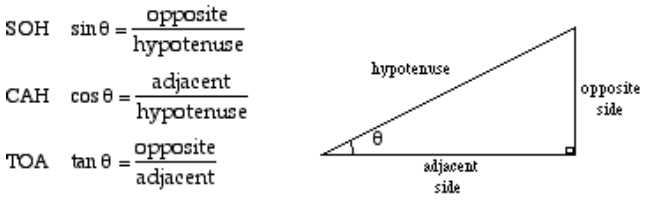
\includegraphics[scale=0.5]{soh-cah-toa.png}
\end{figure}

\subsection*{Integration of Rational Functions by Partial Functions}
\emph{TODO}
% See assignment 2
% If degree(numerator) \geq degree(denominator), long divide.
% If still not simple enough to integrate, use partial functions.
% Note: use calculator when doing long division to verify

\subsection*{Improper Integrals} % section 7.8
There are \textbf{2 types} of improper integrals; a definite integral where:
\begin{enumerate}
\item the interval is infinite
\item $f$ has an infinite discontinuity in $[a,b]$
\end{enumerate}

\subsubsection*{Infinite Intervals} % see assignment 2 & notes
\setcounter{equation}{0}
\begin{align}
\int_a^\infty f(x)\,dx &= \lim_{t \to \infty} \int_a^t f(x)\,dx \\
\int_{-\infty}^b f(x)\,dx &= \lim_{t \to -\infty} \int_t^b f(x)\,dx \\
\int_{-\infty}^\infty f(x)\,dx &= \int_{-\infty}^0 f(x)\,dx + \int_0^\infty f(x)\,dx
\end{align}

\subsubsection*{Discontinuous Integrand}
Some integrals are discontinuous at a limit or between limits.
We approximate the integral near the discontinuity.\\
The improper integral $\int_a^b f(x)\,dx$ is called \textbf{convergent} if the
corresponding limit exists and \textbf{divergent} otherwise.

\begin{enumerate}[(a)]
\item $f$ is continous on $[a,b)$ and discontinous at $b$
  \begin{equation*}
  \int_a^b f(x)\,dx = \lim_{t \to b^-} \int_a^t f(x)\,dx
  \end{equation*}
\item $f$ is continous on $(a,b]$ and discontinous at $a$
  \begin{equation*}
  \int_a^b f(x)\,dx = \lim_{t \to a^+} \int_t^b f(x)\,dx
  \end{equation*}
\item $f$ has a discontinuity at $c$, where $a < c < b$
  \begin{equation*}
  \int_a^b f(x)\,dx = \int_a^c f(x)\,dx + \int_c^b f(x)\,dx
  \end{equation*}
  If \textbf{both} $\int_a^c f(x)\,dx$ and $\int_c^b f(x)\,dx$ are convergent,
  then so is $\int_a^b f(x)\,dx$.
\end{enumerate}

\noindent \framebox{\textbf{Tip:} use calculator to approximate} \\
Approach from left: $t \rightarrow 2^-$, type $1.\bar{9}$ \\
Approach from right: $t \rightarrow 2^+$, type $2.\bar{0}1$

\subsection*{Strategy for Integration} % section 7.5 -- see notes
\emph{TODO}

\section{Further Applications of Integration} % Chapter 8
\emph{TODO}

\subsection*{Arc Length (length of curve)}
\begin{equation}
L = \int_a^b \sqrt{1 + [f'(x)]^2} \, dx
\end{equation}
$L = \int_a^b \sqrt{1 + [f'(x)]^2} \, dx$

\section{Differential Equations} % Chapter 9
A differential equation is an equation that contains an unknown function and one or more
of its derivatives.
Differential equations typically arise in the process of mathematically modeling some real-world
phenomenon, and are therefore an important application of calculus.

\subsection*{Modeling with Differential Equations} % Section 9.1
The growth rate, $\frac{dP}{dt}$, of a population is proportional to the population size
$\Rightarrow \frac{dP}{dt} = kP$. \\
Where $t=$ time, $P=$ \# of individuals in population, and $k=$ proportionality constant.\\
In general, a solution is a \emph{family} of functions of the form $P(t) = C e^{kt}$,
where $C$ is any real number greater than 0. \\
The \textbf{order} of a differential equation is the order of the highest
derivative that occurs in the equation.\\
When asked to \emph{solve} a differential equation, you are expected to find all possible
solutions of the equation.
\\
\subsubsection*{Initial-value problem}
\begin{enumerate}
\item Find a solution of the differential equation that satisfies the \textbf{initial condition}.
\item Plug the initial condition into the general solution to solve for $C$.
\item Finally, write the specific solution by plugging $C$'s value into the general solution.
\end{enumerate}

\emph{TODO: example}


\subsection*{Separable Equations} % Section 9.3
Separable equations are a type of first-order differential equation that can be solved explicitly,
and are of the form
\begin{equation*}
\frac{dy}{dx} = g(x)f(y)
\mbox{  or  }
\frac{dy}{dx} = \frac{g(x)}{f(y)}
\end{equation*}

\noindent To solve, you must separate the functions on the RHS side and rewrite them in differential form.
\\If you are given an equation in the form of $y'$, rewrite it in Leibniz notation $\frac{dy}{dx}$.\\
\textbf{Summary:} Get all $y$'s on one side, all $x$'s on the other, integrate both sides, 
solve for $y$ and $C$ if given an initial value condition.
\begin{eqnarray*}
\frac{dy}{dx} &=& g(x)f(y) \: \Rightarrow \:
dy = g(x)f(y)\,dx \: \Rightarrow \:
\frac{dy}{f(y)} = g(x)\,dx \: \Rightarrow \:
\int \frac{dy}{f(y)} = \int g(x)\,dx
\\
\frac{dy}{dx} &=& \frac{g(x)}{f(y)} \: \Rightarrow \:
f(y)\,dy = g(x)\,dx \: \Rightarrow \:
\int f(y)\,dy = \int g(x)\,dx
\end{eqnarray*}

\emph{TODO: example}\\

\subsection*{Linear Equations} % Section 9.5
A first-order linear (non-separable) differential equation that can be put in the form
\begin{equation*}
y' + P(x)y = Q(x)
\end{equation*}

\begin{enumerate}
\item Put the equation in the form $y' + P(x)y = Q(x)$.
\item Find the integrating factor $I(x) = e^{\int P(x)\, dx}$.
\item Multiply both sides by the integrating factor $I(x)(y' + P(x)y) = I(x)Q(x)$.
\item Rewrite the LHS as $(y \, e^{\int P(x)\, dx})'$.
\item Integrate both sides.
\item Solve for $y$, by dividing through $e^{f(x)}$ or multiplying by $e^{-f(x)}$
(because $e^{f(x)} \cdot e^{-f(x)} = 1$).
\end{enumerate}

%For example,
%\begin{eqnarray*}
%xy' + y = 2x \: (x \neq 0) \\
%y' = \frac{1}{x}y = 2 \\
%\end{eqnarray*}
%\emph{TODO}\\

\section{Newton's Law of Cooling}
The rate of change of the temperature of an object is proportional to the
difference between its own temperature and the ambient temperature (i.e. the
temperature of its surroundings).

\begin{equation}
T(t) = T_{env} + (T_0 - T_{env}) \, e^{-kt}
\end{equation}
$T(t) = $ temperature of an object at time $t$ (in min) \\
$T(0) = T_0 = $ initial temperature of the object \\
$T_{env} = $ temperature of the environment \\
\\
Plug in the given values, rearrange, and solve for $k$. \\
Plug in $k$ and solve for $t$ in a similar manner if needed. \\
Hint: $\ln(e^u) = u$.

\section{Infinite Sequences and Series} % Chapter 11
\emph{TODO:} short description

\subsection*{Sequences} % Section 11.1
A sequence $\{a_n\}$ has the \textbf{limit} $L$
\begin{equation*}
\lim_{n \to \infty} a_n = L \quad \mbox{ or } \quad a_n \to L \mbox{ as } n \to \infty
\end{equation*}
\\
If $\lim_{n \to \infty} a_n$ exists ($L$ is finite), then
$\{a_n\}$ \textbf{converges} (or is \textbf{convergent}), otherwise
it \textbf{diverges} (or is \textbf{divergent}).
\\
\\
Limit Laws for Sequences % pg 693 - TODO: redo as eqnarray?
\begin{itemize}
\item $\lim_{n \to \infty} (a_n \pm b_n) = \lim_{n \to \infty} a_n \, \pm \, \lim_{n \to \infty} b_n$
\item $\lim_{n \to \infty} C\,a_n= C \lim_{n \to \infty} a_n$
(e.g. $\lim_{n \to \infty} \sqrt{\frac{n^2}{n^2 + 1}} = \sqrt{ \lim_{n \to \infty} \frac{n^2}{n^2 + 1}}$)
\item $\lim_{n \to \infty} a_n b_n = \lim_{n \to \infty} a_n \cdot \lim_{n \to \infty} b_n$
\item $\lim_{n \to \infty} \frac{a_n}{b_n} = \dfrac{\lim_{n \to \infty} a_n}{\lim_{n \to \infty} b_n}
\quad(\lim_{n \to \infty} b_n \neq 0)$
\item $\lim_{n \to \infty} a_n^{\;p}= [\lim_{n \to \infty} a_n]^p
\quad(p > 0,\: a_n > 0)$
\end{itemize}

% TODO: squeeze theorem - pg 694

\noindent If a sequence has terms with alternating signs, the equation $a_n$ will include
a multiplication by $(-1)^n$.\\

\noindent For a sequence that's a rational function (i.e. $ \lim_{n \to \infty} \frac{a_n}{b_n}$)
you would have to (long) divide it to tell what the limit is.
\textbf{Shortcut:} ignore constants and divide by highest degree of the denominator.

\begin{enumerate}[(a)]
\item degree numerator == degree denonimator $\Rightarrow L =$ coefficients
\begin{equation*}
\mbox{e.g.} \quad \lim_{n \to \infty} \frac{2n^2 + 3n - 1}{5n^2 + n} = \frac{2}{5}
\mbox{ (convergent)}
\end{equation*}

\item degree numerator $>$ degree denonimator $\Rightarrow L = \infty$ or $-\infty$
\begin{equation*}
\mbox{e.g.} \quad \lim_{n \to \infty} \frac{n^2 + 1}{3n + 2}
= \lim_{n \to \infty} \frac{n + \frac{1}{n}}{3 + \frac{2}{n}}
\approx \lim_{n \to \infty} \frac{n}{1} = \infty
\mbox{ (divergent)}
\end{equation*}

\item degree numerator $<$ degree denonimator $\Rightarrow L = 0$
\begin{equation*}
\mbox{e.g.} \quad \lim_{n \to \infty} \frac{3n^7}{5n^8 + 10n + 2}
\approx \lim_{n \to \infty} \frac{1}{n} = 0
\mbox{ (convergent)}
\end{equation*}

\item indeterminate form $\left(0^0,\, \frac{0}{0},\, 1^\infty,\, \infty - \infty,\, \frac{\infty}{\infty},\,0 \cdot \infty,\, \infty^0\right) \Rightarrow$ change $n$ to $x$ and apply L'Hopital's rule
\begin{equation*}
\mbox{e.g.} \quad \lim_{n \to \infty} \frac{n+1}{e^n} \Rightarrow \lim_{x \to \infty} \frac{x+1}{e^x}
= \lim_{x \to \infty} \frac{1}{e^x} = 0 
\mbox{ (convergent)}
\end{equation*}
\end{enumerate}

\subsection*{Series} % Section 11.2
A series is a summation of a sequence.
\begin{equation*}
a_1 + a_2 + a_3 + \cdots + a_n + \cdots = \sum_{n=1}^\infty a_n = \sum a_n
\end{equation*}
\begin{equation}
\sum_{n=1}^\infty a_n = \lim_{n \to \infty} S_n = S
\end{equation}
where $S_n$ is the expression for the sum of the first $n$, and $S$ is the sum of the series.

\noindent If $S_n$ isn't given, you have to find it,
which is usually not easy, unless it's a geometric series. \\


\noindent The \textbf{geometric series}
\begin{equation*}
\sum_{n=1}^\infty ar^{n-1} = a + ar + ar^2 + \cdots
\end{equation*}
\textbf{converges} to $\dfrac{a}{1-r}$ if $|r| < 1$, otherwise \textbf{diverges}.
\\
\\
\noindent \framebox{\textbf{Tip:} write out the series as $a + ar + ar^2 + \cdots$ to find $a$ and $r$}
\\

\noindent Sometimes you need to \textbf{split the series} into multiple geometric series
of the form $\sum a\,r^{n-1}$, for example:
\begin{align*}
\sum \left(\frac{8}{10}\right)^{n-1} - \left(\frac{3}{10}\right)^n
= \sum \left(\frac{8}{10}\right)^{n-1} - \sum \left(\frac{3}{10}\right) \left(\frac{3}{10}\right)^{n-1}\\
\frac{1}{3} + \frac{2}{9} + \frac{1}{27} + \frac{2}{81} + \frac{1}{243} + \frac{2}{729} + \cdots
= \frac{1}{3} + \frac{1}{27} + \frac{1}{243} + \cdots + \frac{2}{9} + \frac{2}{81} + \frac{2}{729} + \cdots
\end{align*}


\noindent \framebox{\textbf{Reminder:} if $\sum a_n$ and $\sum b_n$ are convergent,
then so are $\sum (a_n \pm b_n)$, $\sum C\, a_n$, and $\sum C\, b_n$}

\subsection*{Infinite Series Summary}
% TODO: see reference sheet for infinite series
% TODO: include examples of what to use when
\subsubsection*{Geometric Series}
\emph{TODO}
\subsection*{$p$-series}
\emph{TODO}
\subsection*{Divergence Test} % aka test for divergence
\emph{TODO}
\subsection*{Integral Test}
\emph{TODO}
\subsection*{Comparison Test}
\emph{TODO}
\subsection*{Limit Comparison Test} % use when comparison test condition fails
\emph{TODO}
\subsection*{Alternating Series Test}
\emph{TODO}
\subsection*{Ratio Test} % if one fails, so does the other
\emph{TODO}
\subsection*{Root Test}
\emph{TODO}

\section{Algebra Tips} % See back of Tan's Calculus book
\emph{TODO}

\begin{eqnarray*} % Maybe use tabular instead? But will be inline math.
x^{\frac{1}{2}} = \sqrt(x) \\
\sqrt[4]{x} = x^{\frac{1}{4}} \\
(a^x)^y = a^{xy} \\
a^x \cdot a^y = a^{x+y} \\
\ln a + \ln b = \ln ab \\
\ln a - \ln b = \ln \frac{a}{b} \\
\ln(e^x) = x \\
e^{\ln(x)} = x \\
\dfrac{\frac{a}{b}}{\frac{c}{d}} = \frac{a}{b} \times \frac{d}{c} = \dfrac{\frac{d}{c}}{\frac{b}{a}}
\end{eqnarray*}
  

\section{Tools}
\subsection*{Maple Classic}
\emph{TODO:} post images of stuff from assignments
\subsection*{WolframAlpha}
\begin{itemize}
\item $\frac{d}{dx} \sqrt[4]{x} \Rightarrow$ ``d/dx fourth root of x'' or ``d/dx x\char`\^(1/4)''
\item $\int \sqrt{\cos(x)} \sin^3(x)\,dx \Rightarrow$ ``integral sqrt(cosx) sin\char`\^3x''
\item $\int_a^b \cos2x \, dx \Rightarrow$ ``integral cos2x from a to b''
\item $\int_{-2}^2 (4+y^2) - (2y^2) \, dy \Rightarrow$ ``area between x=2y\char`\^2 and x=4+y\char`\^2''
\item $\int_a^b \sqrt{1 + (f'(x))^2}\,dx \Rightarrow$ ``length f(x) from a to b''
\item $\pi \int_a^b \left(f(x)^2 - g(x)^2\right)\,dx \Rightarrow$ ``pi * integral...''
\item $\{(1+\frac{1}{n})^n\} \rightarrow a_n = (1+\frac{1}{n})^n \Rightarrow$ ``limit (1+1/n)\char`\^n as n-$>$infinity''
\item Check an infinite series for convergence $\rightarrow$ ``series  sum ( $a_n$ ) from n = 1 to infty''
\end{itemize}

\end{document}